\subsection*{I. Système de Cramer}
\begin{enumerate}
 \item Le point fondamental est que l'espace des formes bilinéaires antisymétriques sur un plan est un espace vectoriel de dimension $1$ (cours). Il existe donc un réel $\lambda$ tel que 
 \begin{displaymath}
   \det_{(\overrightarrow{u},\overrightarrow{v})} = \lambda \det_{(\overrightarrow{i},\overrightarrow{j})}
 \end{displaymath}
Pour calculer ce $\lambda$, on prend la valeur pour la famille  $(\overrightarrow{i},\overrightarrow{j})$. On en déduit
\begin{displaymath}
  \det_{(\overrightarrow{u},\overrightarrow{v})} = 
  \det_{(\overrightarrow{u},\overrightarrow{v})}((\overrightarrow{i},\overrightarrow{j})
  \det_{(\overrightarrow{i},\overrightarrow{j})}
\end{displaymath}
On obtient la relation demandée en prenant la valeur pour la famille $(\overrightarrow{u},\overrightarrow{v})$.\newline
Soit $(\lambda, \mu)$ les coordonnées de $\overrightarrow{w}$:
\begin{displaymath}
  \overrightarrow{w}= \lambda \overrightarrow{u} + \mu \overrightarrow{u}
  \Rightarrow
\left\lbrace  
\begin{aligned}
  \det_{(\overrightarrow{i},\overrightarrow{j})}(\overrightarrow{w},\overrightarrow{v})=&
  \lambda \det_{(\overrightarrow{i},\overrightarrow{j})}(\overrightarrow{u},\overrightarrow{v})\\
  \det_{(\overrightarrow{i},\overrightarrow{j})}(\overrightarrow{u},\overrightarrow{w})=&
  \mu \det_{(\overrightarrow{i},\overrightarrow{j})}(\overrightarrow{u},\overrightarrow{v})
\end{aligned}
\right. 
\end{displaymath}
Les coordonnées de $\overrightarrow{w}$ dans $(\overrightarrow{u},\overrightarrow{v})$ sont donc
\begin{displaymath}
  \left( \frac{\det_{(\overrightarrow{i},\overrightarrow{j})}(\overrightarrow{w},\overrightarrow{v})}
              {\det_{(\overrightarrow{i},\overrightarrow{j})}(\overrightarrow{u},\overrightarrow{v})},
         \frac{\det_{(\overrightarrow{i},\overrightarrow{j})}(\overrightarrow{u},\overrightarrow{w})}
              {\det_{(\overrightarrow{i},\overrightarrow{j})}(\overrightarrow{u},\overrightarrow{v})}
  \right) 
\end{displaymath}

 \item Comme $\overrightarrow{u}$ et $\overrightarrow{v}$ sont dans $\Z\overrightarrow{i} + \Z\overrightarrow{j}$, une inclusion est évidente:
 \begin{displaymath}
   \Z\overrightarrow{u} + \Z\overrightarrow{v} \subset \Z\overrightarrow{i} + \Z\overrightarrow{j}
 \end{displaymath}
Il s'agit donc de pouver l'équivalence
 \begin{displaymath}
   \Z\overrightarrow{i} + \Z\overrightarrow{j} \subset \Z\overrightarrow{u} + \Z\overrightarrow{v}
   \Leftrightarrow \det_{(\overrightarrow{i},\overrightarrow{j})}(\overrightarrow{u},\overrightarrow{v})\in\left\lbrace -1, +1\right\rbrace 
 \end{displaymath}
Supposons que le déterminant soit $\pm1$.\newline
Les formules de Cramer de la question précédente exprimant les coordonnées dans $(\overrightarrow{u},\overrightarrow{v})$ d'un vecteur $w\in \Z\overrightarrow{i} + \Z\overrightarrow{j}$ montrent l'inclusion demandée car les déterminants au numérateur sont des entiers.\newline
Réciproquement, supposons l'inclusion.\newline
Les coordonnées des vecteurs $\overrightarrow{i}$ et $\overrightarrow{j}$ dans $(\overrightarrow{u},\overrightarrow{v})$ sont entiers. On en déduit que les deux déterminants de la relation
 \begin{displaymath}
   \det_{(\overrightarrow{u},\overrightarrow{v})}(\overrightarrow{i},\overrightarrow{j})
   \det_{(\overrightarrow{i},\overrightarrow{j})}(\overrightarrow{u},\overrightarrow{v}) = 1
 \end{displaymath}
sont des entiers. Ils sont donc tous les deux dans $\left\lbrace -1, 1\right\rbrace$.
\end{enumerate}

\subsection*{II. Triangles élémentaires}
\begin{enumerate}
 \item D'après le cours sur les déterminants,
 \begin{displaymath}
   S = \frac{1}{2} \det(\overrightarrow{AB},\overrightarrow{AC})
 \end{displaymath}
On peut se permettre de ne pas écrire l'indice $(\overrightarrow{i},\overrightarrow{j})$ précisant la base dans laquelle on considère le déterminant car elle est orthonormée directe. La forme bilinéaire déterminant est la même pour toutes ces bases. Comme le déterminant prend une valeur entière car les coordonnées sont entières, l'aire d'un triangle entier est un multiple de $\frac{1}{2}$. 

 \item \'Ecrivons les coordonnées des côtés du parallélograme et du triangle
\begin{multline*}
  P\in (AB)\Leftrightarrow Y(P)=0,\hspace{0.5cm}
  P\in (CD)\Leftrightarrow Y(P)=1,\hspace{0.5cm}\\
  P\in (AC)\Leftrightarrow X(P)=0,\hspace{0.5cm}
  P\in (BD)\Leftrightarrow X(P)=1,\hspace{0.5cm}\\
  P\in (BC)\Leftrightarrow X(P)+Y(P)-1=0,\hspace{0.5cm}
\end{multline*}
On en déduit les systèmes d'inéquations des surfaces polygonales
\begin{align*}
\text{parallélograme}& &0\leq X(P) \leq 1 , \; 0\leq Y(P) \leq 1 \\
\text{triangle}& &0\leq X(P) , \; 0\leq Y(P), \; X(P) + Y(P) - 1 \leq 0
\end{align*}
 
 \item Notons $\overrightarrow{u} = \overrightarrow{AB}$ et $\overrightarrow{v} = \overrightarrow{AC}$:
\begin{displaymath}
  S = \frac{1}{2} \Rightarrow \det_{(\overrightarrow{i},\overrightarrow{j})}(\overrightarrow{u},\overrightarrow{v})=1
\end{displaymath}
On en déduit avec I.2. que, pour tout point $P$ entier, $X(P)$ et $Y(P)$ sont des entiers. Alors, en utilisant 2.,
\begin{displaymath}
\left. 
\begin{aligned}
  X(P)\in& \N \\ Y(P)\in& \N \\ X(P)+Y(P)\leq& 1
\end{aligned}
\right\rbrace 
\Rightarrow
\left\lbrace 
\begin{aligned}
  (X(P)=1, Y(P)=0) \text{ ou }&\\ (X(P)=0, Y(P)=1) \text{ ou }&\\ (X(P)=0, Y(P)=0)
\end{aligned}
\right.  
\end{displaymath}
c'est à dire $P\in\left\lbrace A, B, C\right\rbrace$. 

 \item
 \begin{enumerate}
   \item Soit $Q$ un point entier. Approchons ses coordonnées dans la base associée au triangle par des parties entières. 
Définissons $P$ par:
\begin{displaymath}
  X(P) = X(Q) - \lfloor X(Q) \rfloor, \hspace{0.5cm} 
  Y(P) = Y(Q) - \lfloor Y(Q) \rfloor
\end{displaymath}
Si au moins une des coordonnées $X(Q)$, $Y(Q)$ n'est pas entière, alors au moins une des coordonnées $X(P)$, $Y(P)$ n'est pas nulle donc
   \begin{displaymath}
     0\leq X(P) < 1, \hspace{0.5cm} 0\leq Y(P) < 1 , \hspace{0.5cm} X(P)Y(P) = 0
   \end{displaymath}
De plus $P$ est un point entier car $\overrightarrow{QP} \in \Z \overrightarrow{i} +  \Z \overrightarrow{j}$.
Le point $P'$ est entier même si $X(P)$ et $Y(P)$ ne le sont pas car
\begin{displaymath}
  \overrightarrow{PP'} = \overrightarrow{u} + \overrightarrow{v} - \overrightarrow{AP} \in \Z\overrightarrow{i}+\Z\overrightarrow{j}
\end{displaymath}
Remarquons que $0\leq X(P') \leq1$ et $0\leq Y(P') \leq 1$ donc $P'$ est dans le parallélograme.
   \item Pour un triangle entier $(A,B,C)$, d'après la question précédente, s'il existe un point entier $Q$ dont les coordonnées relatives au triangle ne sont pas entières, il existe des points entiers $P$ et $P'$ dans le parallélograme. De plus
\begin{displaymath}
  X(P') + Y(P') - 1 = -\left( X(P) + Y(P) -1\right) 
\end{displaymath}
donc au moins un des deux est dans le triangle $(A,B,C)$. Par définition de $P$ au moins une de ses coordonnées est dans $]0,1[$ donc il n'est pas un sommet, par définition de $P'$, aucune de ses coordonnées n'est nulle donc il n'est pas un sommet.\newline
Autrement dit: s'il existe un point entier dont les coordonnées dans le repère du triangle ne sont pas entières, alors le triangle $(A,B,C)$ n'est pas élémentaire. Par contraposition, si $(A,B,C)$ est élémentaire alors tous les points entiers sont à coordonnées entières dans le repère du triangle ce qui entraine
\begin{displaymath}
  \Z\overrightarrow{i}+\Z\overrightarrow{j} \subset \Z\overrightarrow{u}+\Z\overrightarrow{v}
\end{displaymath}
On conclut avec I.1., le déterminant vaut $1$ puis II.1., l'aire du triangle est $\frac{1}{2}$.


 \end{enumerate}

\end{enumerate}

\subsection*{III. Aires et comptages}
\begin{enumerate}
 \item Un triangle élémentaire $\mathcal T$ ne contient aucun point entier sauf ses sommets et son aire est $\frac{1}{2}$ donc
\begin{displaymath}
\left. 
\begin{aligned}
i(\mathcal T)=& 0 \\ l(\mathcal T) =& 3 
\end{aligned}
\right\rbrace 
\Rightarrow
i(\mathcal T)+\frac{1}{2}l(\mathcal T)-1=\frac{3}{2}-1=\frac{1}{2} = \text{ aire du triangle}
\end{displaymath}

 \item Pour toute surface polygonale $\mathcal P$, définissons $\alpha$ par 
\begin{displaymath}
\alpha(\mathcal P)=i(\mathcal P)+\frac{1}{2}l(\mathcal P)-1  
\end{displaymath}
Montrons que sous les hypothèses de la question
\begin{displaymath}
 \alpha(\mathcal P_1 \cup \mathcal P_2)=\alpha(\mathcal P_1 )+\alpha(\mathcal P_2)
\end{displaymath}
Supposons que les deux surfaces aient en commun une ligne polygonale comprenant $p$ points entiers. Les deux extrémités sont sur le bord. On peut alors écrire
\begin{align*}
 &i(\mathcal P_1 \cup \mathcal P_2)=i(\mathcal P_1)+i(\mathcal P_2)+p-2 &\times 1\\
 &l(\mathcal P_1 \cup \mathcal P_2)=l(\mathcal P_1)+l(\mathcal P_2)-2p +2 &\times \frac{1}{2}
\end{align*}
et combiner avec les coefficients indiqués
\begin{multline*}
  \alpha(\mathcal P_1 \cup \mathcal P_2)-1=\alpha(\mathcal P_1)-1+\alpha(\mathcal P_2)-1+(p-2)+\frac{1}{2}(-2p+2) \\
\Rightarrow
 \alpha(\mathcal P_1 \cup \mathcal P_2)=\alpha(\mathcal P_1)+\alpha(\mathcal P_2)
\end{multline*}
Comme l'aire vérifie la même formule d'additivité, l'égalité entre les deux fonctions se propage à $\mathcal P_1 \cup \mathcal P_2$.

 \item Tout triangle entier, s'il n'est pas élémentaire se décompose en triangles entiers comme dans la question précédente. 
Si le triangle contient un point entier intérieur, on le décompoe en trois triangles entiers. Si le triangle contient un point entier sur un côté, on le décompose en deux. On peut poursuivre le processus tant que les triangles ne sont pas élémentaires. Tout triangle entier se décompose donc en triangles élémentaires qui sont de Pick.
\begin{figure}[!ht]
 \centering
 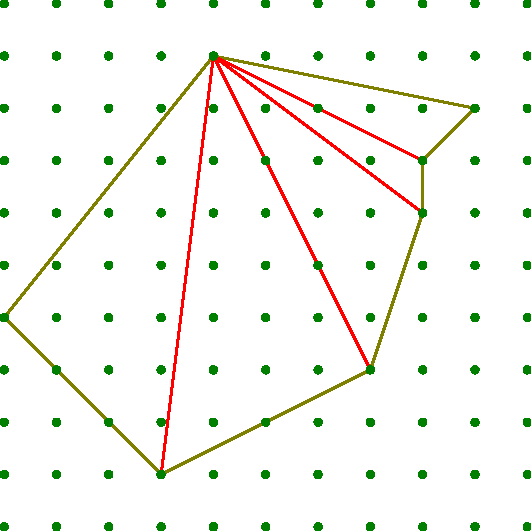
\includegraphics[width=7cm]{./Cpick_1.pdf}
 \caption{Décomposition en triangles entiers}
 \label{fig:Cpick_1}
\end{figure}

 \item La surface polygonale proposée se décompose en triangles (figure \ref{fig:Cpick_1}) vérifiant la condition de la question 2. Elle est donc de Pick et son aire se calcule en comptant les points. On trouve
\begin{displaymath}
 37 + \frac{1}{2}\,10 -1 =41
\end{displaymath}

\end{enumerate}
